% This section contains notes on "Configure Microsoft Azure Active Directory for workloads" relevant subjects %
\subsubsection{Application management}
\begin{figure}[!h]
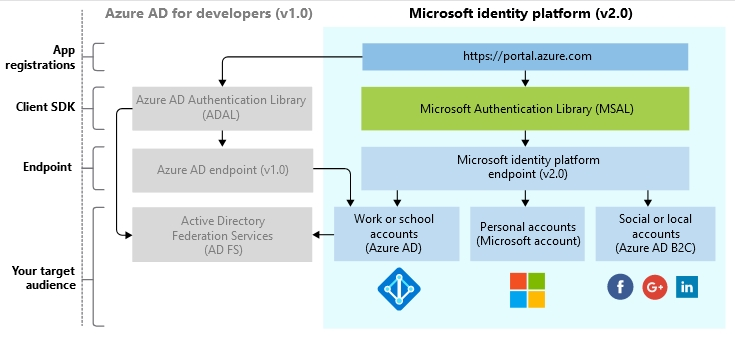
\includegraphics[width=1\textwidth]{microsoft-identity-platform.jpg}
\caption{Microsoft identity platform}
\end{figure}

\textbf{Permission / scope} \\
Azure AD defines two kinds of permissions:
\begin{itemize}
\item Delegated. Applications with signed in users. Can be either user or admin consent. The application is granted permission to act as the singed-in user when making requests. \\ Effective permissions are the \textit{least} privileged intersection of the delegated permissions for the application itself (through consent) and the privileges of the signed-in user. Within organizations, the privileges of the signed-in user may be determined by policy or by group membership.
\item Application. Applications without signed in users. Can only be granted by administrator or the user which is stated as owner of the resource application. \\ Effective permissions is the full set of privileges granted by the permission.
\end{itemize}
Effective permissions are the permissions that your app will have when making requests to an API.

\textbf{Consent} \\
Applications in Azure AD rely on consent in order to gain access to necessary resources or APIs.
\begin{itemize}
\item Static user. All required permissions are pre-specified in the app's configuration in Azure portal.
\item Dynamic user. Additional permissions can be obtained when using the application. Users are prompted for additional permissions as required.
\item Admin user. Required for specific high-privilege permissions. Must be granted ahead of time, cannot be dynamic. 
\end{itemize}

\textbf{Trivia and quirks} 
\begin{enumerate}
\item Microsoft identity platform is an evolution of the Azure Active Directory developer platform
\item Preview versions of MSAL libraries have the same level of support as production versions of MSAL and ADAL.
\item Microsoft identity platform (v2.0) endpoint is now OIDC certified
\end{enumerate}

\subsubsection{User management}
When using groups for managing the following methods should be considered:
\begin{description}
\item[Self-service group management.] When Azure AD groups are managed by group owners instead of IT administrators.
\item[Dynamic group membership.] When a series of rules govern membership in Azure AD groups, by automatically add or remove user accounts. \begin{enumerate} \item If a new user account matches all the rules for the group, it becomes a member. \item If a user account isn’t a member of the group, but its attributes change so that it matches all the rules for the group, it becomes a member of that group. \item If a user account is a member of the group, but its attributes change so that it no longer matches all the rules for the group, it is removed as a member of the group. \end{enumerate}
\item[Group-based licensing.] Automating the assigning, and removal, of licenses based on group membership.
\end{description}

\textbf{Trivia and quirks} 
\begin{enumerate}
\item Self-service group management is available only for Azure AD security and Office 365 groups. \textit{It is not available for mail-enabled groups, distribution lists, or any group that has been synchronized from your on-premises Active Directory Domain Services (AD DS).}
\end{enumerate}

\subsubsection{Conditional Access}
\textbf{Application and enforcement}
\begin{enumerate}
\item All policies that apply must be satisfied.
\item Phase 1 : All policies are evaluated and all access controls that aren't satisfied are collected.
\item Phase 2 : Prompted to satisfy the requirements you haven't met \textit{in order}.
	\begin{enumerate}
	\item Multi-factor authentication
	\item Compliant device
	\item Hybrid Azure AD joined device
	\item Approved client app
	\end{enumerate}
\end{enumerate}
The Conditional Access framework provides you with a great configuration flexibility. However, great flexibility also means that you should carefully review each configuration policy before releasing it to avoid undesirable results.  \\

When new policies are ready for your environment, deploy them in phases:
\begin{enumerate}
\item Apply a policy to a small set of users and verify it behaves as expected.
\item When you expand a policy to include more users. Continue to exclude all administrators from the policy to ensure that they still have access and can update a policy if a change is required.
\item Apply a policy to all users only if necessary.
\end{enumerate}

\begin{itemize}
\item As a first step, you should evaluate your policy using the what if tool.
\item Create a user account that is:
	\begin{itemize}
	\item Dedicated to policy administration
	\item Excluded from all your policies
	\end{itemize}
\end{itemize}

\subsubsection{Identity protection}
Identity Protection seeks to accomplish three key tasks:
\begin{enumerate}
\item Automate the detection and remediation of identity-based risks.
\item Investigate risks using data in the portal.
\item Export risk detection data to third-party utilities for further analysis.
\end{enumerate}

\textbf{Risk detection} \\
Risk detections in Azure AD Identity Protection include any identified suspicious actions related to user accounts in the directory.
\begin{itemize}
\item User
	\begin{itemize}
	\item Leaked Credentials. \textit{This risk detection indicates that the user's valid credentials have been leaked.}
	\item Azure AD threat intelligence. \textit{Microsoft’s internal and external threat intelligence sources have identified a known attack pattern.}
	\end{itemize}
\item Sign-in
	\begin{itemize}
	\item Atypical travel. \textit{Sign in from an atypical location based on the user’s recent sign-ins.}
	\item Anonymous IP address. \textit{Sign in from an anonymous IP address (for example: Tor browser, anonymizer VPNs).}
	\item Unfamiliar sign-in properties. \textit{Sign in with properties we‘ve not seen recently for the given user.}
	\item Malware linked IP address. \textit{Sign in from a malware linked IP address.}
	\item Admin confirmed user compromised. \textit{This detection indicates an admin has selected 'Confirm user compromised' in the Risky users UI or using riskyUsers API.}
	\item Malicious IP address. \textit{This detection indicates sign-in from a malicious IP address. An IP address is considered malicious based on high failure rates because of invalid credentials received from the IP address or other IP reputation sources.}
	\end{itemize}
\end{itemize}

\textbf{Investigating risk}
\begin{itemize}
\item Risky users \\
	\begin{tabular}{p{7cm}p{7cm}}
	\underline{Information}
		\begin{itemize}
		\item Users at risk
		\item Details about detections
		\item History of risky sign-ins
		\item Risk history
		\end{itemize} &
	\underline{Actions}
		\begin{itemize}
		\item Reset the user password
		\item Confirm user compromise
		\item Dismiss user risk
		\item Block user from signing in
		\item Investigate further using Azure ATP
		\end{itemize}
	\end{tabular}	
\item Risky sign-ins. \textit{The risky sign-ins report contains data for up to the past 30 days.} \\
	\begin{tabular}{p{7cm}p{7cm}}
	\underline{Information}
		\begin{itemize}
		\item Sign-ins indicating risk
		\item Real-time and aggregate risk levels associated with sign-in attempts
		\item Detection types triggered
		\item Conditional Access policies applied
		\item MFA details
		\item Device information
		\item Application information
		\item Location information
		\end{itemize} &
	\underline{Actions}
		\begin{itemize}
		\item Confirm sign-in compromise
		\item Confirm sign-in safe
		\end{itemize}
	\end{tabular}
\item Risk detections \\
	\begin{tabular}{p{7cm}p{7cm}}
	\underline{Information}
		\begin{itemize}
		\item Information about each risk detection including type
		\item Other risks triggered at the same time
		\item Sign-in attempt location
		\item Link out to more detail from Microsoft Cloud App Security (MCAS)
		\end{itemize} &
	\underline{Actions}
		\begin{itemize}
		\item Return to either user risk or sign-in report and take action there
		\end{itemize}
	\end{tabular}
\end{itemize}
The three reports are found in the Azure portal > Azure Active Directory > Security.
\begin{figure}[!h]
\centering
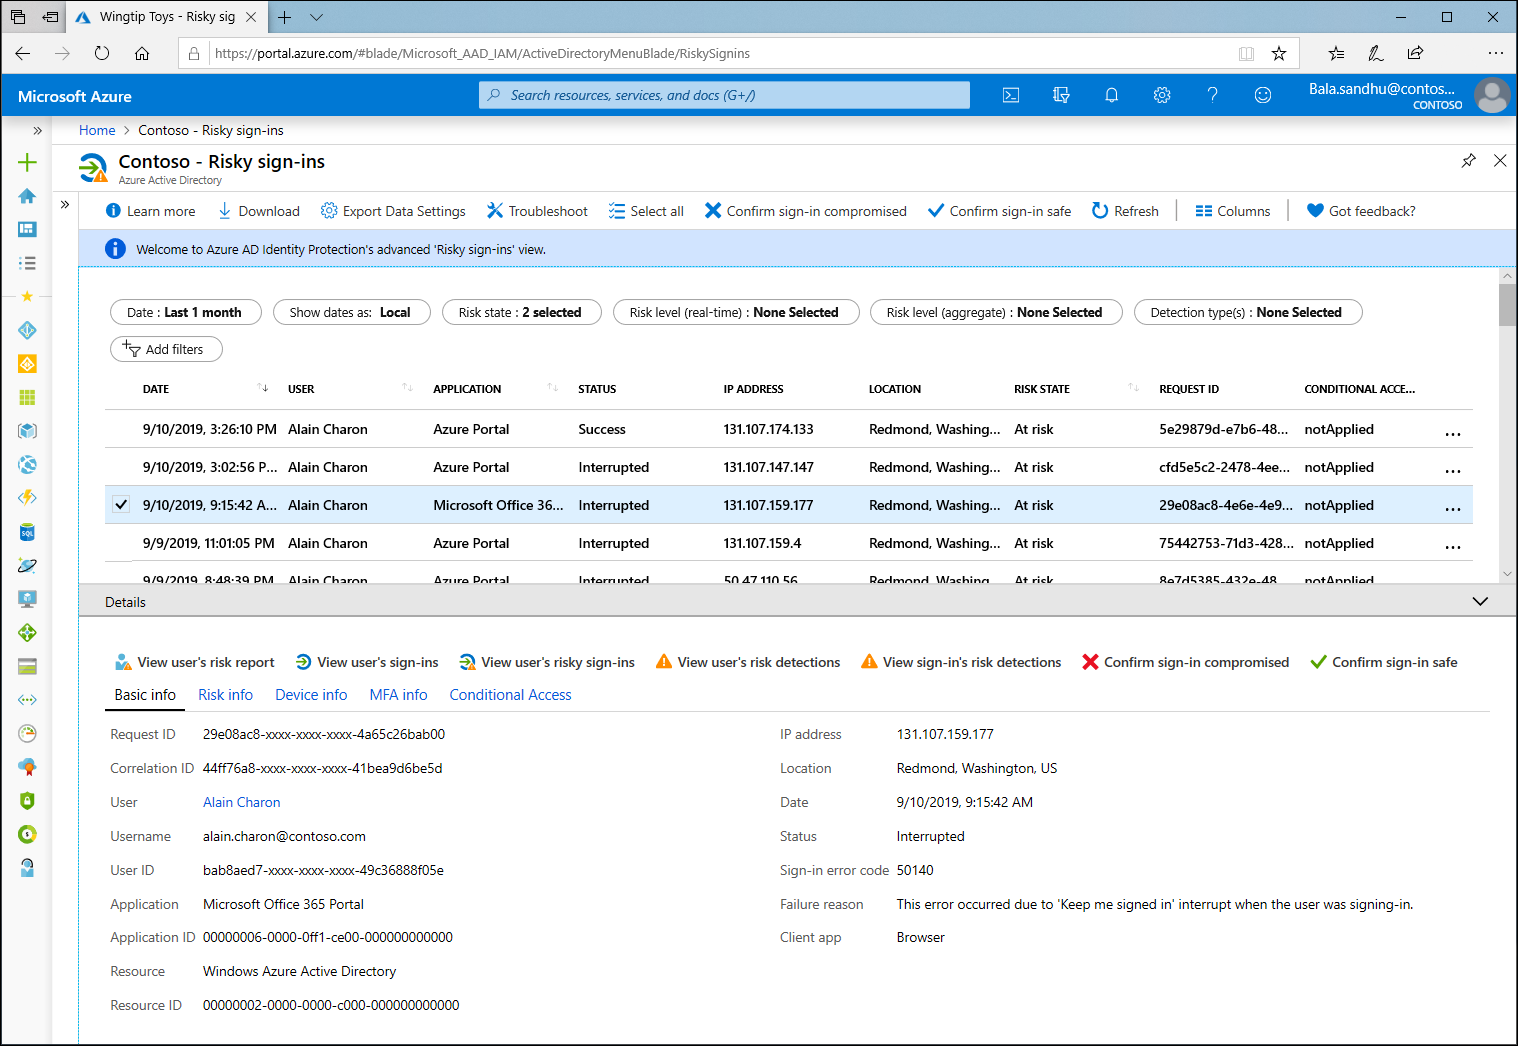
\includegraphics[width=0.8\textwidth]{identity-protection-risky-sign-ins-report.png}
\caption{Identify protection risky sign-ins report}
\end{figure}

\textbf{Remediation}
\begin{enumerate}
\item Technical tools
	\begin{enumerate}
	\item Azure Multi-Factor Authentication
	\item Reset their password using self-service password reset
	\item Blocking until an administrator takes action
	\end{enumerate}
\item Policies
	\begin{enumerate}
	\item MFA registration policy. \textit{Can help organizations roll out MFA using a Conditional Access policy requiring registration at sign-in.}
	\item Sign-in risk policy. \textit{Analyzes signals from each sign-in, both real-time and offline, and calculates a risk score based on the probability that the sign-in wasn't performed by the user. If risk is detected, users can perform multi-factor authentication to self-remediate and close the risky sign-in event to prevent unnecessary noise.}
	\item User risk policy. \textit{Calculate what it believes is normal for a user's behaviour and use that to base decisions for their risk. If risk is detected, users can perform self-service password reset to self-remediate and close the user risk event to prevent unnecessary noise.}
	\end{enumerate}
\end{enumerate}

\textbf{License requirements} \\
\begin{tabular}{l p{6cm} c c c}

 &  & Premium P2 & Premium P1 & Basic/Free \\
Risk policies & User risk policy & \cmark & \xmark & \xmark \\
Risk policies & Sign-in risk policy & \cmark & \xmark & \xmark \\
Security reports & Overview & \cmark & \xmark & \xmark \\
Security reports & Risky users & \cmark & Limited & Limited \\
Security reports & Risky sign-ins & \cmark & Limited & Limited \\
Security reports & Risk detections & \cmark & Limited & \xmark \\
Notifications & Users at risk detected alerts & \cmark & \xmark & \xmark \\
Notifications & Weekly digest & \cmark & \xmark & \xmark \\
	& MFA registration policy & \cmark & \xmark & \xmark \\
\end{tabular}

\textbf{Users role with Identity Protection access}
\begin{enumerate}
\item Security Reader
\item Security Operator
\item Security Administrator
\item Global Reader
\item Global Administrator
\end{enumerate}

\subsubsection{Azure AD Connect}
\textbf{Wizards} 
\begin{itemize}
\item Express. Requires high level of privileges and does not require creating users or configuring permissions. Requires two accounts a) AD DS Enterprise Administrator and b) Azure AD Global Administrator.

\item Custom. It is used in all cases where the express installation option does not satisfy your deployment or topology.
\end{itemize}

\textbf{Accounts} 
\begin{itemize}
\item Synchronisation
	\begin{itemize}
	\item AD DS Connector account: \\ Used to read/write information to Windows Server Active Directory.
	\item ADSync service account: \\ Used to run the synchronization service and access the SQL database.
	\item Azure AD Connector account: \\ Used to write information to Azure AD.
	\end{itemize}
\item Installation
	\begin{itemize}
	\item Local Administrator account: \\ The administrator who is installing Azure AD Connect and who has local Administrator permissions on the machine.
	\item AD DS Enterprise Administrator account: \\ Optionally used to create the "AD DS Connector account" above.
	\item Azure AD Global Administrator account: \\ Used to create the Azure AD Connector account and configure Azure AD. \\ After installation this account should be changed from Global Administrator role to the \textit{Directory Synchronization Accounts} role.
	\item SQL SA account (optional): \\ Used to create the ADSync database when using the full version of SQL Server. This account could be the same account as the Enterprise Administrator. 
	\end{itemize}
\end{itemize}
\begin{figure}[!h]
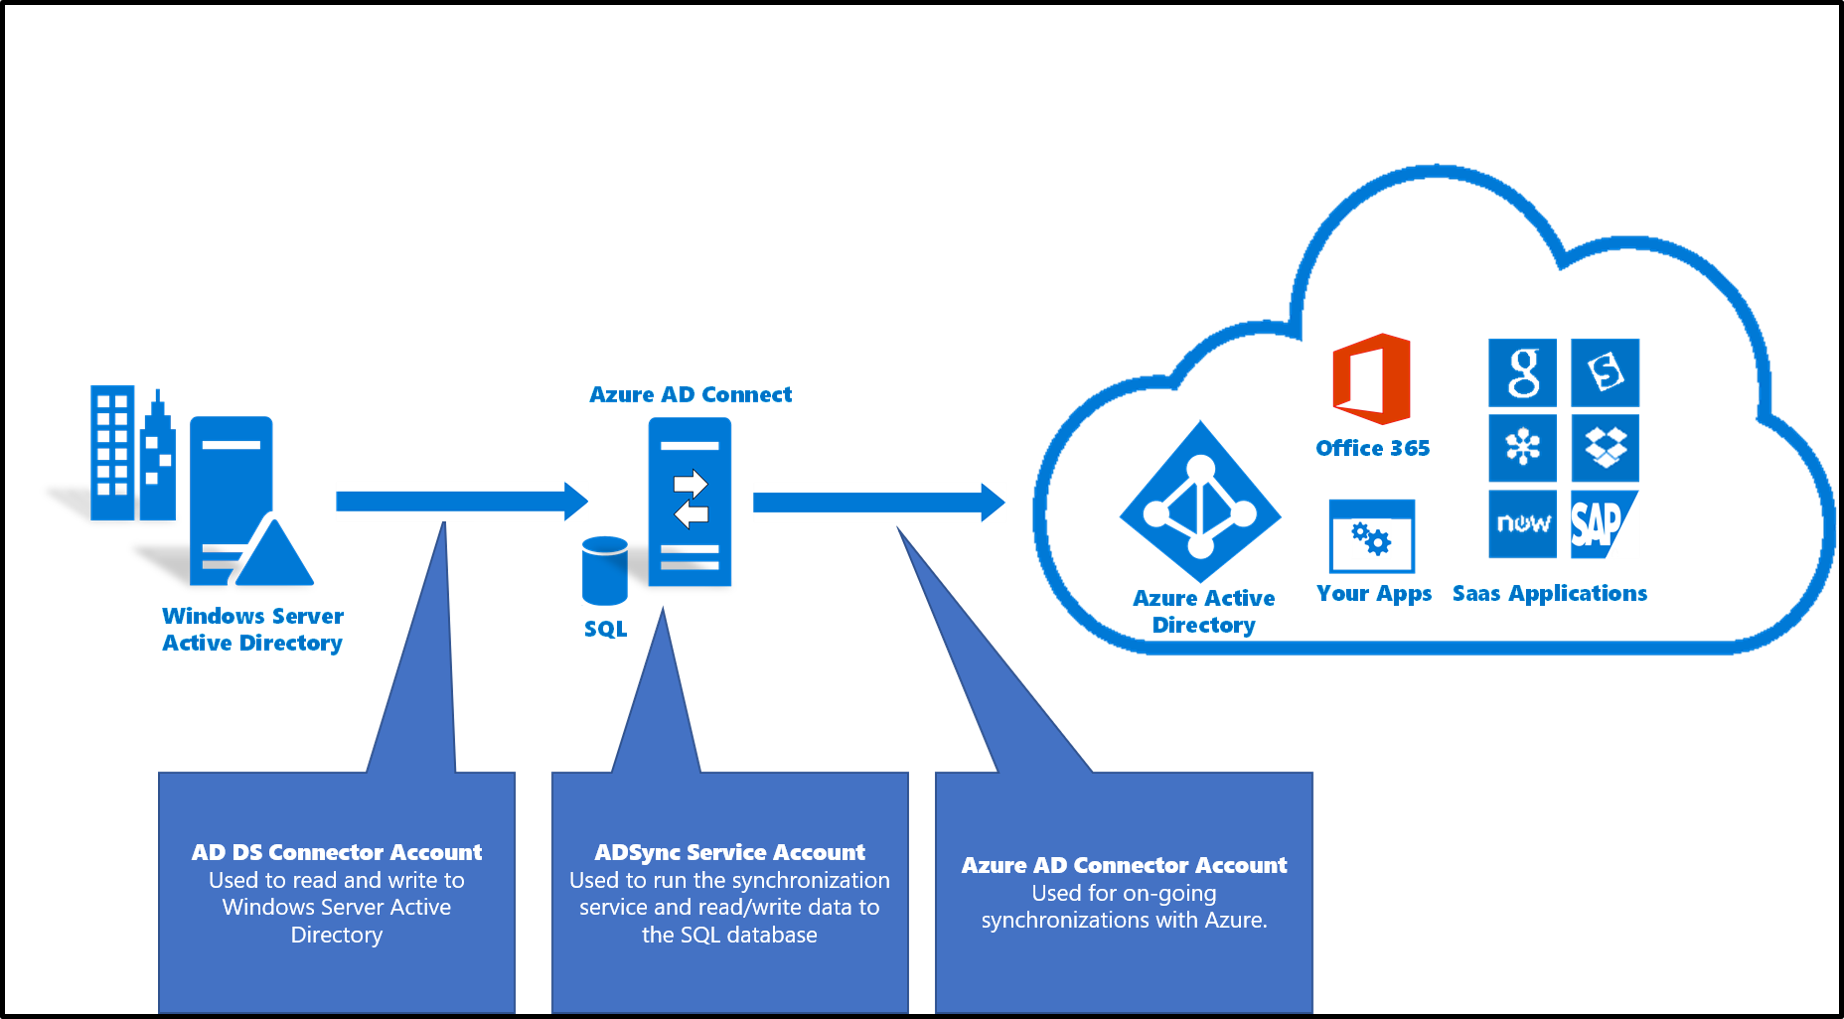
\includegraphics[width=1\textwidth]{azure-ad-connect-account.png}
\caption{Accounts used for Azure AD Connect}
\label{fig:azure-connect-accounts}
\end{figure}

\textbf{Components}
\begin{itemize}
\item SQL Server 2012 Express, LocalDB instance
\item User sign-in scheme
	\begin{itemize}
	\item Password Hash Sync. \textit{The users passwords are synchronized to Azure AD as a password hash and authentication occurs in the cloud.}
	\item Pass-through Authentication. \textit{The users password is passed through to the on-premises Active Directory domain controller to be validated.}
	\item Federation with AD FS. \textit{The users are redirected to their on-premises AD FS instance to sign in and authentication occurs on-premises.}
	\item Federation with PingFederate. \textit{ The users are redirected to their on-premises PingFederate instance to sign in and authentication occurs on-premises.}
	\item Do not configure. \textit{No user sign-in feature is installed and configured. Choose this option if you already have a 3rd party federation server or another existing solution in place.}
	\item [Option] Enable Single Sign on. \textit{Provides a single sign on experience for desktop users on the corporate network. For Hash or Pass-through.}
	\end{itemize}
\end{itemize}